%% Source Template:
%% Copyright (C) 2014 by Pascal Richter, Elena Botoeva, Richard Barnard, and Dirk Surmann
%% 
%% This file may be distributed and/or modified under the
%% conditions of the LaTeX Project Public License, either
%% version 2.0 of this license or (at your option) any later
%% version. The latest version of this license is in:
%% 
%% http://www.latex-project.org/lppl.txt
%% 
%% and version 2.0 or later is part of all distributions of
%% LaTeX version 2013/12/01 or later.
%% 

\documentclass[20pt, a1paper, portrait, margin=0mm, innermargin=10mm,
               blockverticalspace=10mm,colspace=5mm, subcolspace=0mm]
               {tikzposter}

% Choose Layout
\usetheme{Autumn}

% Additonal packages
\usepackage{wrapfig}
\usepackage{floatflt}
\usepackage{multicol}
\usepackage{placeins}
\usepackage[T1]{fontenc}
\usepackage{natbib}

% Set block style
\useblockstyle[titlewidthscale=1, bodywidthscale=1, titlecenter,
    titleoffsetx=0pt, titleoffsety=0pt, bodyoffsetx=0pt, bodyoffsety=25pt,
    bodyverticalshift=0pt, roundedcorners=5, linewidth=0.4cm,
    titleinnersep=10mm, bodyinnersep=10mm]{Default}

\usetitlestyle[titletoblockverticalspace=10mm]{Filled}

\tikzposterlatexaffectionproofoff


% Header
\title{\textcolor{colorThree}{\fontsize{2.3cm}{1em}\selectfont 
       Searching for signals in noise}}

\author{Gregory Ashton, supervised by D.I. Jones \& R. Prix \\
    {\Large G.Ashton@soton.ac.uk}}

\institute{University of Southampton }

\begin{document}

 % Title block with title, author, logo, etc.
\maketitle


 %\block{Introduction}{
%}
\begin{columns}
 % FIRST column
\newcommand{\mycolwidth}{0.5}
\column{\mycolwidth}
\block[]{I: Motivations}{
Astrophysics contains a huge number of interesting observed phenomena, let alone
those that we have yet to see. The problem we often have is that 
that our observations are in a low signal to noise regime; this can mean
several models can explain the observed data. 

In this poster we discuss a method for quantitatively assesing how well several
models fit some data. The aim being to decide, eventually, given the observed 
data which astrophysical model do we think is most likely.

}



 % SECOND column
\column{\mycolwidth}

\block{II: Bayesian Data Analysis}{
While many methods exist for comparing some models, an intuitive approach can
be found by using Bayes rule
\begin{equation}
    P(A|B) = P(B|A) \frac{P(A)}{P(B)}
\end{equation}
where by $P(A|B)$ we mean "The probability of $A$, given that $B$ \emph{is} 
true". The $A$ and $B$ here can be anything.

}

\end{columns}

\block[]{III: Example}{

\begin{wrapfigure}[8]{l}{0.33\linewidth}
    \vspace{-10mm}
\begin{tikzfigure}
    \centering
    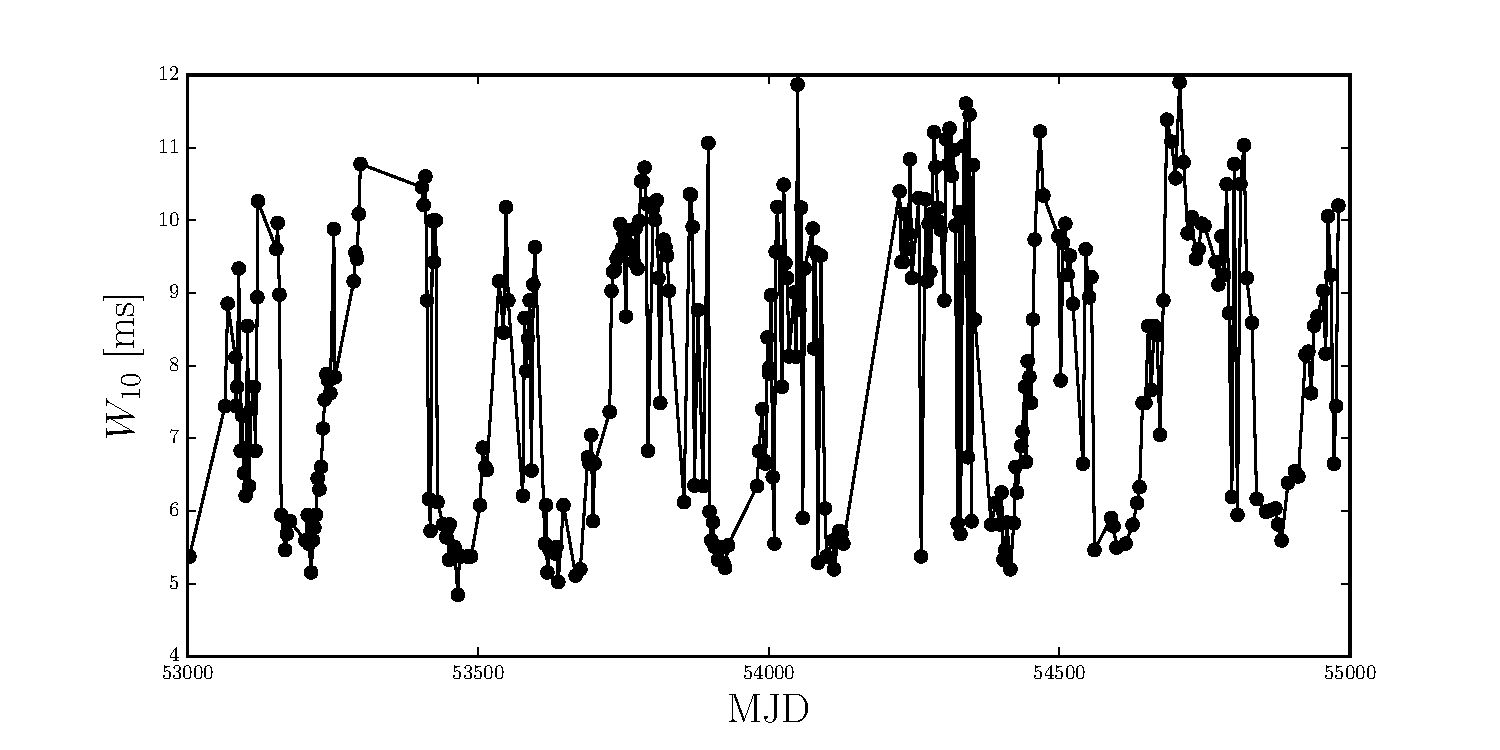
\includegraphics[width=0.3\textwidth]{img/raw_data}
\end{tikzfigure}
\end{wrapfigure}

To illustrate how we can apply Bayesian data analysis consider the data
shown in the figure on the left. This is a plot of the measured beam width
of pulsar B1828-11 showing a distinct periodic behaviour. This data was 
originally published in figure 5 of \citet{Lyne2010}, we are thankful
to the original authors for allowing us access to this data.

Prior to this paper, slow periodic modulation of the spindown was cited as
evidence for precession in this pulsar. Clearly the beam width is also being 
modulated at this same time-scale. The authors argue that the beam width is
not smoothly varying between, but instead \emph{switching}. This has important
implications for neutron star physics.

While there are many ways to model this beam width, we can start by asking a
simple question: is the observed data best explained by a square wave model, or
a smoothly varying sinusoid. While neither of this captures all of the physics
it at least addresses the issue of whether the modulation is smooth or instantaneous.

}

\begin{columns}

\column{0.5}
\block[]{V: Parameter estimation}{
}

\column{0.5}
\block[]{VI: Model comparison}{
}
\end{columns}

\end{document}



\endinput
%%
